\section{Lokaler Repeater Betrieb} \label{sec:lokal}
Eigentlich ist es das Ziel von DMR, transparent gegenüber Repeatern zu sein. Das heißt, es spielt keine Rolle für den Teilnehmer welchen Repeater er benutzt. Er wird immer die selben Teilnehmer erreichen können. Dieses Konzept wird aber durch die Sprechgruppen mit den Nummern $8$ und $9$ durchbrochen.
 
\begin{figure}[!ht]
 \centering
 \documentclass{standalone}
\usepackage{tikz}
\usetikzlibrary{shapes.geometric}
\newcommand{\repeater}[3]{%
 \node ({#1}) at ({#2}) {%
  \begin{tikzpicture}%
   \draw [black,thick] (-.25,0) -- (0,0.5) -- (0.25,0) -- (-0.25,0);%
   \draw [black,thick,domain=-45:225] plot ({0.2*cos(\x)}, {0.5+0.2*sin(\x)});%
   \draw [black,thick,domain=-45:225] plot ({0.4*cos(\x)}, {0.5+0.4*sin(\x)});%
   \node (xxx) at (0,-.2) {{#3}};%
  \end{tikzpicture}%
 } %
}

\newcommand{\activerepeater}[3]{%
 \node ({#1}) at ({#2}) {%
  \begin{tikzpicture}%
   \draw [black,thick] (-.25,0) -- (0,0.5) -- (0.25,0) -- (-0.25,0);%
   \draw [red,thick,domain=-45:225] plot ({0.2*cos(\x)}, {0.5+0.2*sin(\x)});%
   \draw [red,thick,domain=-45:225] plot ({0.4*cos(\x)}, {0.5+0.4*sin(\x)});%
   \node (xxx) at (0,-.2) {{#3}};%
  \end{tikzpicture}%
 } %
}


\newcommand{\user}[3]{%
 \node ({#1}) at ({#2}) {%
  \begin{tikzpicture}%
   \draw [black,fill=black] (-.25,0) -- (0,0.5) -- (0.25,0) -- (-0.25,0);%
   \draw [black,fill=black] (0,.5) circle (.2); %
   \node (xxx) [text width=0.6cm, align=center] at (-.35cm,-.4) {{#3}};%
  \end{tikzpicture}%
 } %
}

\newcommand{\activeuser}[3]{%
 \node ({#1}) at ({#2}) {%
  \begin{tikzpicture}%
   \draw [red,fill=red] (-.25,0) -- (0,0.5) -- (0.25,0) -- (-0.25,0);%
   \draw [red,fill=red] (0,.5) circle (.2); %
   \node (xxx) [text width=0.6cm, align=center] at (-.35cm,-.4) {{#3}};%
  \end{tikzpicture}%
 } %
}

\begin{document}
 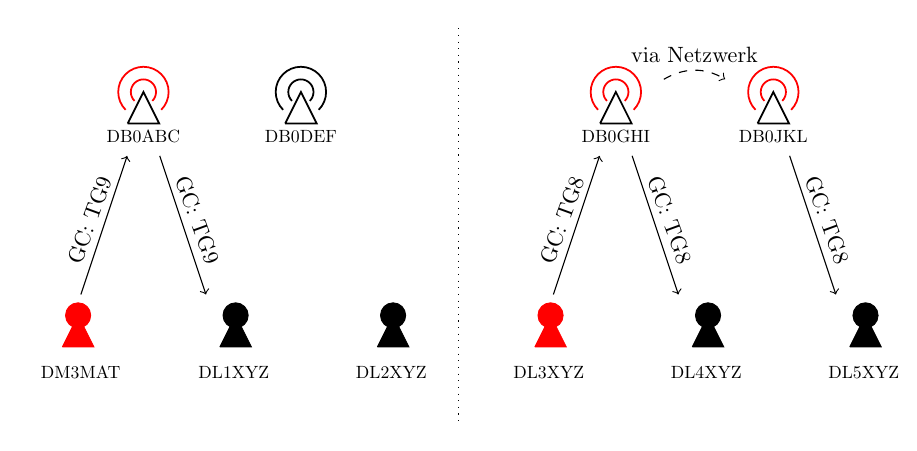
\begin{tikzpicture}[every node/.style={scale=.8}]
  \activeuser{u1}{ 0,0}{DM3MAT};
  \user{u2}{ 2,0}{DL1XYZ};	
  \user{u3}{ 4,0}{DL2XYZ};	
  \draw[dotted] (5,4) -- (5,-1);
  \activeuser{u4}{ 6,0}{DL3XYZ};
  \user{u5}{ 8,0}{DL4XYZ};
  \user{u6}{10,0}{DL5XYZ};
  \activerepeater{R1}{1,3}{DB0ABC};
  \repeater{R2}{3,3}{DB0DEF};
  \activerepeater{R3}{7,3}{DB0GHI};
  \activerepeater{R4}{9,3}{DB0JKL};
  \draw[->] (u1) -- node[above,rotate=70]{GC: TG9} (R1);
  \draw[->] (R1) -- node[above,rotate=-70]{GC: TG9} (u2);
  \draw[->] (u4) -- node[above,rotate=70]{GC: TG8} (R3);
  \draw[->] (R3) -- node[above,rotate=-70]{GC: TG8} (u5);
  \draw[->] (R4) -- node[above,rotate=-70]{GC: TG8} (u6);
  \path[->] (R3) edge[dashed,bend left] node[above]{via Netzwerk} (R4);
 \end{tikzpicture}
\end{document}

 \caption{Beispiel mit zwei Regionen (links \& rechts) mit je zwei Repeatern.} \label{fig:tg9tg8}
\end{figure}

Die Sprechgruppe 9 (kurz TG9) ist die sogenannte \emph{lokale} Sprechgruppe. Gruppenrufen zu dieser Sprechgruppe werden nicht über das Netzwerk weitergeleitet, sonder nur lokal vom jeweiligen Repeater ausgesandt. Dieser Fall ist in Abbildung \ref{fig:tg9tg8} links dargestellt. Hier sendet DM3MAT einen Gruppenruf zur TG9 über den Repeater DB0ABC. Dieser Ruf wird nicht an weitere Repeater übertragen und ist somit nur in der Umgebung des Repeaters zu hören. DL1XYZ befindet sich in der Nähe des Repeaters und kann den Ruf empfangen, wenn er sein Funkgerät so konfiguriert hat, dass es Gruppenrufe an die TG9 empfängt.    

Die Sprechgruppe 8 (TG8) ist die sogenannte \emph{regionale} Sprechgruppe. Ein Gruppenruf zu dieser Sprechgruppe wird meist durch alle Repeater innerhalb einer Region ausgesandt. Welche Repeater zu einer Region gehören und wie groß diese Region letztendlich ist, entscheiden die Administratoren der jeweiligen Repeater. Sie entscheiden ob ihre Repeater zu einer Region gehören sollen oder nicht. Im Beispiel in Abbildung \ref{fig:tg9tg8} rechts, sendet DL3XYZ einen Gruppenruf zur Sprechgruppe 8 an den Repeater DB0GHI, dieser sendet diesen Gruppenruf selbst aus und leitet ihn an alle Repeater im regionalen Verbund (auch \adef{Cluster}) weiter. In diesem Fall auch an den Repeater DB0JKL. Somit können alle Teilnehmer in der Region diesen Gruppenruf empfangen, solange sie ihre Funkgeräte entsprechend konfiguriert haben. In diesem Beispiel empfängt somit nicht nur DL4XYZ den Gruppenruf sondern auch DL5XYZ, auch wenn er sich nicht in der Nähe des Repeaters DB0GHI befindet. 